%File: formatting-instructions-latex-2024.tex
%release 2024.0
\documentclass[letterpaper]{article} % DO NOT CHANGE THIS
\usepackage{aaai24}  % DO NOT CHANGE THIS
\usepackage{times}  % DO NOT CHANGE THIS
\usepackage{helvet}  % DO NOT CHANGE THIS
\usepackage{courier}  % DO NOT CHANGE THIS
\usepackage[hyphens]{url}  % DO NOT CHANGE THIS
\usepackage{graphicx} % DO NOT CHANGE THIS
\urlstyle{rm} % DO NOT CHANGE THIS
\def\UrlFont{\rm}  % DO NOT CHANGE THIS
\usepackage{natbib}  % DO NOT CHANGE THIS AND DO NOT ADD ANY OPTIONS TO IT
\usepackage{caption} % DO NOT CHANGE THIS AND DO NOT ADD ANY OPTIONS TO IT
\frenchspacing  % DO NOT CHANGE THIS
\setlength{\pdfpagewidth}{8.5in}  % DO NOT CHANGE THIS
\setlength{\pdfpageheight}{11in}  % DO NOT CHANGE THIS
%
% These are recommended to typeset algorithms but not required. See the subsubsection on algorithms. Remove them if you don't have algorithms in your paper.
\usepackage{algorithm}
\usepackage{algorithmic}
\usepackage{amsfonts}
\usepackage{amsmath}
\usepackage{subfigure}
\usepackage{diagbox}

%
% These are are recommended to typeset listings but not required. See the subsubsection on listing. Remove this block if you don't have listings in your paper.
\usepackage{newfloat}
\usepackage{listings}
\DeclareCaptionStyle{ruled}{labelfont=normalfont,labelsep=colon,strut=off} % DO NOT CHANGE THIS
\lstset{%
	basicstyle={\footnotesize\ttfamily},% footnotesize acceptable for monospace
	numbers=left,numberstyle=\footnotesize,xleftmargin=2em,% show line numbers, remove this entire line if you don't want the numbers.
	aboveskip=0pt,belowskip=0pt,%
	showstringspaces=false,tabsize=2,breaklines=true}
\floatstyle{ruled}
\newfloat{listing}{tb}{lst}{}
\floatname{listing}{Listing}
%
% Keep the \pdfinfo as shown here. There's no need
% for you to add the /Title and /Author tags.
\pdfinfo{
/TemplateVersion (2024.1)
}

% DISALLOWED PACKAGES
% \usepackage{authblk} -- This package is specifically forbidden
% \usepackage{balance} -- This package is specifically forbidden
% \usepackage{color (if used in text)
% \usepackage{CJK} -- This package is specifically forbidden
% \usepackage{float} -- This package is specifically forbidden
% \usepackage{flushend} -- This package is specifically forbidden
% \usepackage{fontenc} -- This package is specifically forbidden
% \usepackage{fullpage} -- This package is specifically forbidden
% \usepackage{geometry} -- This package is specifically forbidden
% \usepackage{grffile} -- This package is specifically forbidden
% \usepackage{hyperref} -- This package is specifically forbidden
% \usepackage{navigator} -- This package is specifically forbidden
% (or any other package that embeds links such as navigator or hyperref)
% \indentfirst} -- This package is specifically forbidden
% \layout} -- This package is specifically forbidden
% \multicol} -- This package is specifically forbidden
% \nameref} -- This package is specifically forbidden
% \usepackage{savetrees} -- This package is specifically forbidden
% \usepackage{setspace} -- This package is specifically forbidden
% \usepackage{stfloats} -- This package is specifically forbidden
% \usepackage{tabu} -- This package is specifically forbidden
% \usepackage{titlesec} -- This package is specifically forbidden
% \usepackage{tocbibind} -- This package is specifically forbidden
% \usepackage{ulem} -- This package is specifically forbidden
% \usepackage{wrapfig} -- This package is specifically forbidden
% DISALLOWED COMMANDS
% \nocopyright -- Your paper will not be published if you use this command
% \addtolength -- This command may not be used
% \balance -- This command may not be used
% \baselinestretch -- Your paper will not be published if you use this command
% \clearpage -- No page breaks of any kind may be used for the final version of your paper
% \columnsep -- This command may not be used
% \newpage -- No page breaks of any kind may be used for the final version of your paper
% \pagebreak -- No page breaks of any kind may be used for the final version of your paperr
% \pagestyle -- This command may not be used
% \tiny -- This is not an acceptable font size.
% \vspace{- -- No negative value may be used in proximity of a caption, figure, table, section, subsection, subsubsection, or reference
% \vskip{- -- No negative value may be used to alter spacing above or below a caption, figure, table, section, subsection, subsubsection, or reference

\setcounter{secnumdepth}{0} %May be changed to 1 or 2 if section numbers are desired.

% The file aaai24.sty is the style file for AAAI Press
% proceedings, working notes, and technical reports.
%

% Title

% Your title must be in mixed case, not sentence case.
% That means all verbs (including short verbs like be, is, using,and go),
% nouns, adverbs, adjectives should be capitalized, including both words in hyphenated terms, while
% articles, conjunctions, and prepositions are lower case unless they
% directly follow a colon or long dash
% \title{Innate-Values-driven Multi-Agent Reinforcement Learning for Social Rewards}
\title{Innate-Values-driven Reinforcement Learning \\ for Cooperative Multi-Agent Systems}

\author{
    %Authors
    % All authors must be in the same font size and format.
    Qin Yang\textsuperscript{\rm 1}\thanks{Qin Yang is the director of the Intelligent Social Systems and Swarm Robotics Lab (IS$^3$R), Computer Science and Information Systems Department, Bradley University, Peoria, IL 61625, USA; Email: is3rlab@gmail.com.}
    % and Ramviyas Parasuraman\textsuperscript{\rm 2}
    % Sunil Issar,\\
    % J. Scott Penberthy,
    % George Ferguson,
    % Hans Guesgen,
    % Francisco Cruz\equalcontrib,
    % Marc Pujol-Gonzalez\equalcontrib
}
\affiliations{
    %Afiliations
    \textsuperscript{\rm 1}Computer Science and Information Systems Department, Braldey University \\
    % If you have multiple authors and multiple affiliations
    % use superscripts in text and roman font to identify them.
    % For example,

    1501 W Bradley Ave, Bradley Hall 195, Peoria, IL 61625, USA\\
    % email address must be in roman text type, not monospace or sans serif
    Email: is3rlab@gmail.com
%
% See more examples next

    % \textsuperscript{\rm 2} Department of Computer Science, University of Georgia \\ Athens, Georgia, U.S
}

%Example, Single Author, ->> remove \iffalse,\fi and place them surrounding AAAI title to use it
\iffalse
\title{My Publication Title --- Single Author}
\author {
    Author Name
}
\affiliations{
    Affiliation\\
    Affiliation Line 2\\
    name@example.com
}
\fi

\iffalse
%Example, Multiple Authors, ->> remove \iffalse,\fi and place them surrounding AAAI title to use it
\title{My Publication Title --- Multiple Authors}
\author {
    % Authors
    First Author Name\textsuperscript{\rm 1,\rm 2},
    Second Author Name\textsuperscript{\rm 2},
    Third Author Name\textsuperscript{\rm 1}
}
\affiliations {
    % Affiliations
    \textsuperscript{\rm 1}Affiliation 1\\
    \textsuperscript{\rm 2}Affiliation 2\\
    firstAuthor@affiliation1.com, secondAuthor@affilation2.com, thirdAuthor@affiliation1.com
}
\fi


% REMOVE THIS: bibentry
% This is only needed to show inline citations in the guidelines document. You should not need it and can safely delete it.
\usepackage{bibentry}
% END REMOVE bibentry

\begin{document}

\maketitle

\begin{abstract}
Innate values describe agents' intrinsic motivations, which reflect their inherent interests and preferences to pursue goals and drive them to develop diverse skills satisfying their various needs. The essence of reinforcement learning (RL) is learning from interaction based on reward-driven (such as utilities) behaviors, much like natural agents. It is an excellent model to describe the innate-values-driven (IV) behaviors of AI agents. Especially in multi-agent systems (MAS), building the awareness of AI agents to balance the group utilities and system costs and satisfy group members' needs in their cooperation is a crucial problem for individuals learning to support their community and integrate human society in the long term. This paper proposes a hierarchical compound intrinsic value reinforcement learning model -- innate-values-driven reinforcement learning termed IVRL to describe the complex behaviors of multi-agent interaction in their cooperation. We implement the IVRL architecture in the StarCraft Multi-Agent Challenge (SMAC) environment and compare the cooperative performance within three characteristics of innate value agents (Coward, Neutral, and Reckless) through three benchmark multi-agent RL algorithms: QMIX, IQL, and QTRAN. The results demonstrate that by organizing individual various needs rationally, the group can achieve better performance with lower costs effectively.

\end{abstract}

\section{Introduction}

In natural systems, motivation is concerned explicitly with the activities of creatures that reflect the pursuit of a particular goal and form a meaningful unit of behavior in this function \cite{heckhausen2018motivation}. Furthermore, intrinsic motivations describe incentives relating to an activity itself, and these incentives residing in pursuing an activity are intrinsic. Intrinsic motivations deriving from an activity may be driven primarily by interest or activity-specific incentives, depending on whether the object of an activity or its performance provides the main incentive \cite{schiefele1996motivation}. They also fall in the category of cognitive motivation theories, which include theories of the mind that tend to be abstracted from the biological system of the behaving organism \cite{merrick2013novelty}.

\begin{figure}[t]
\centering
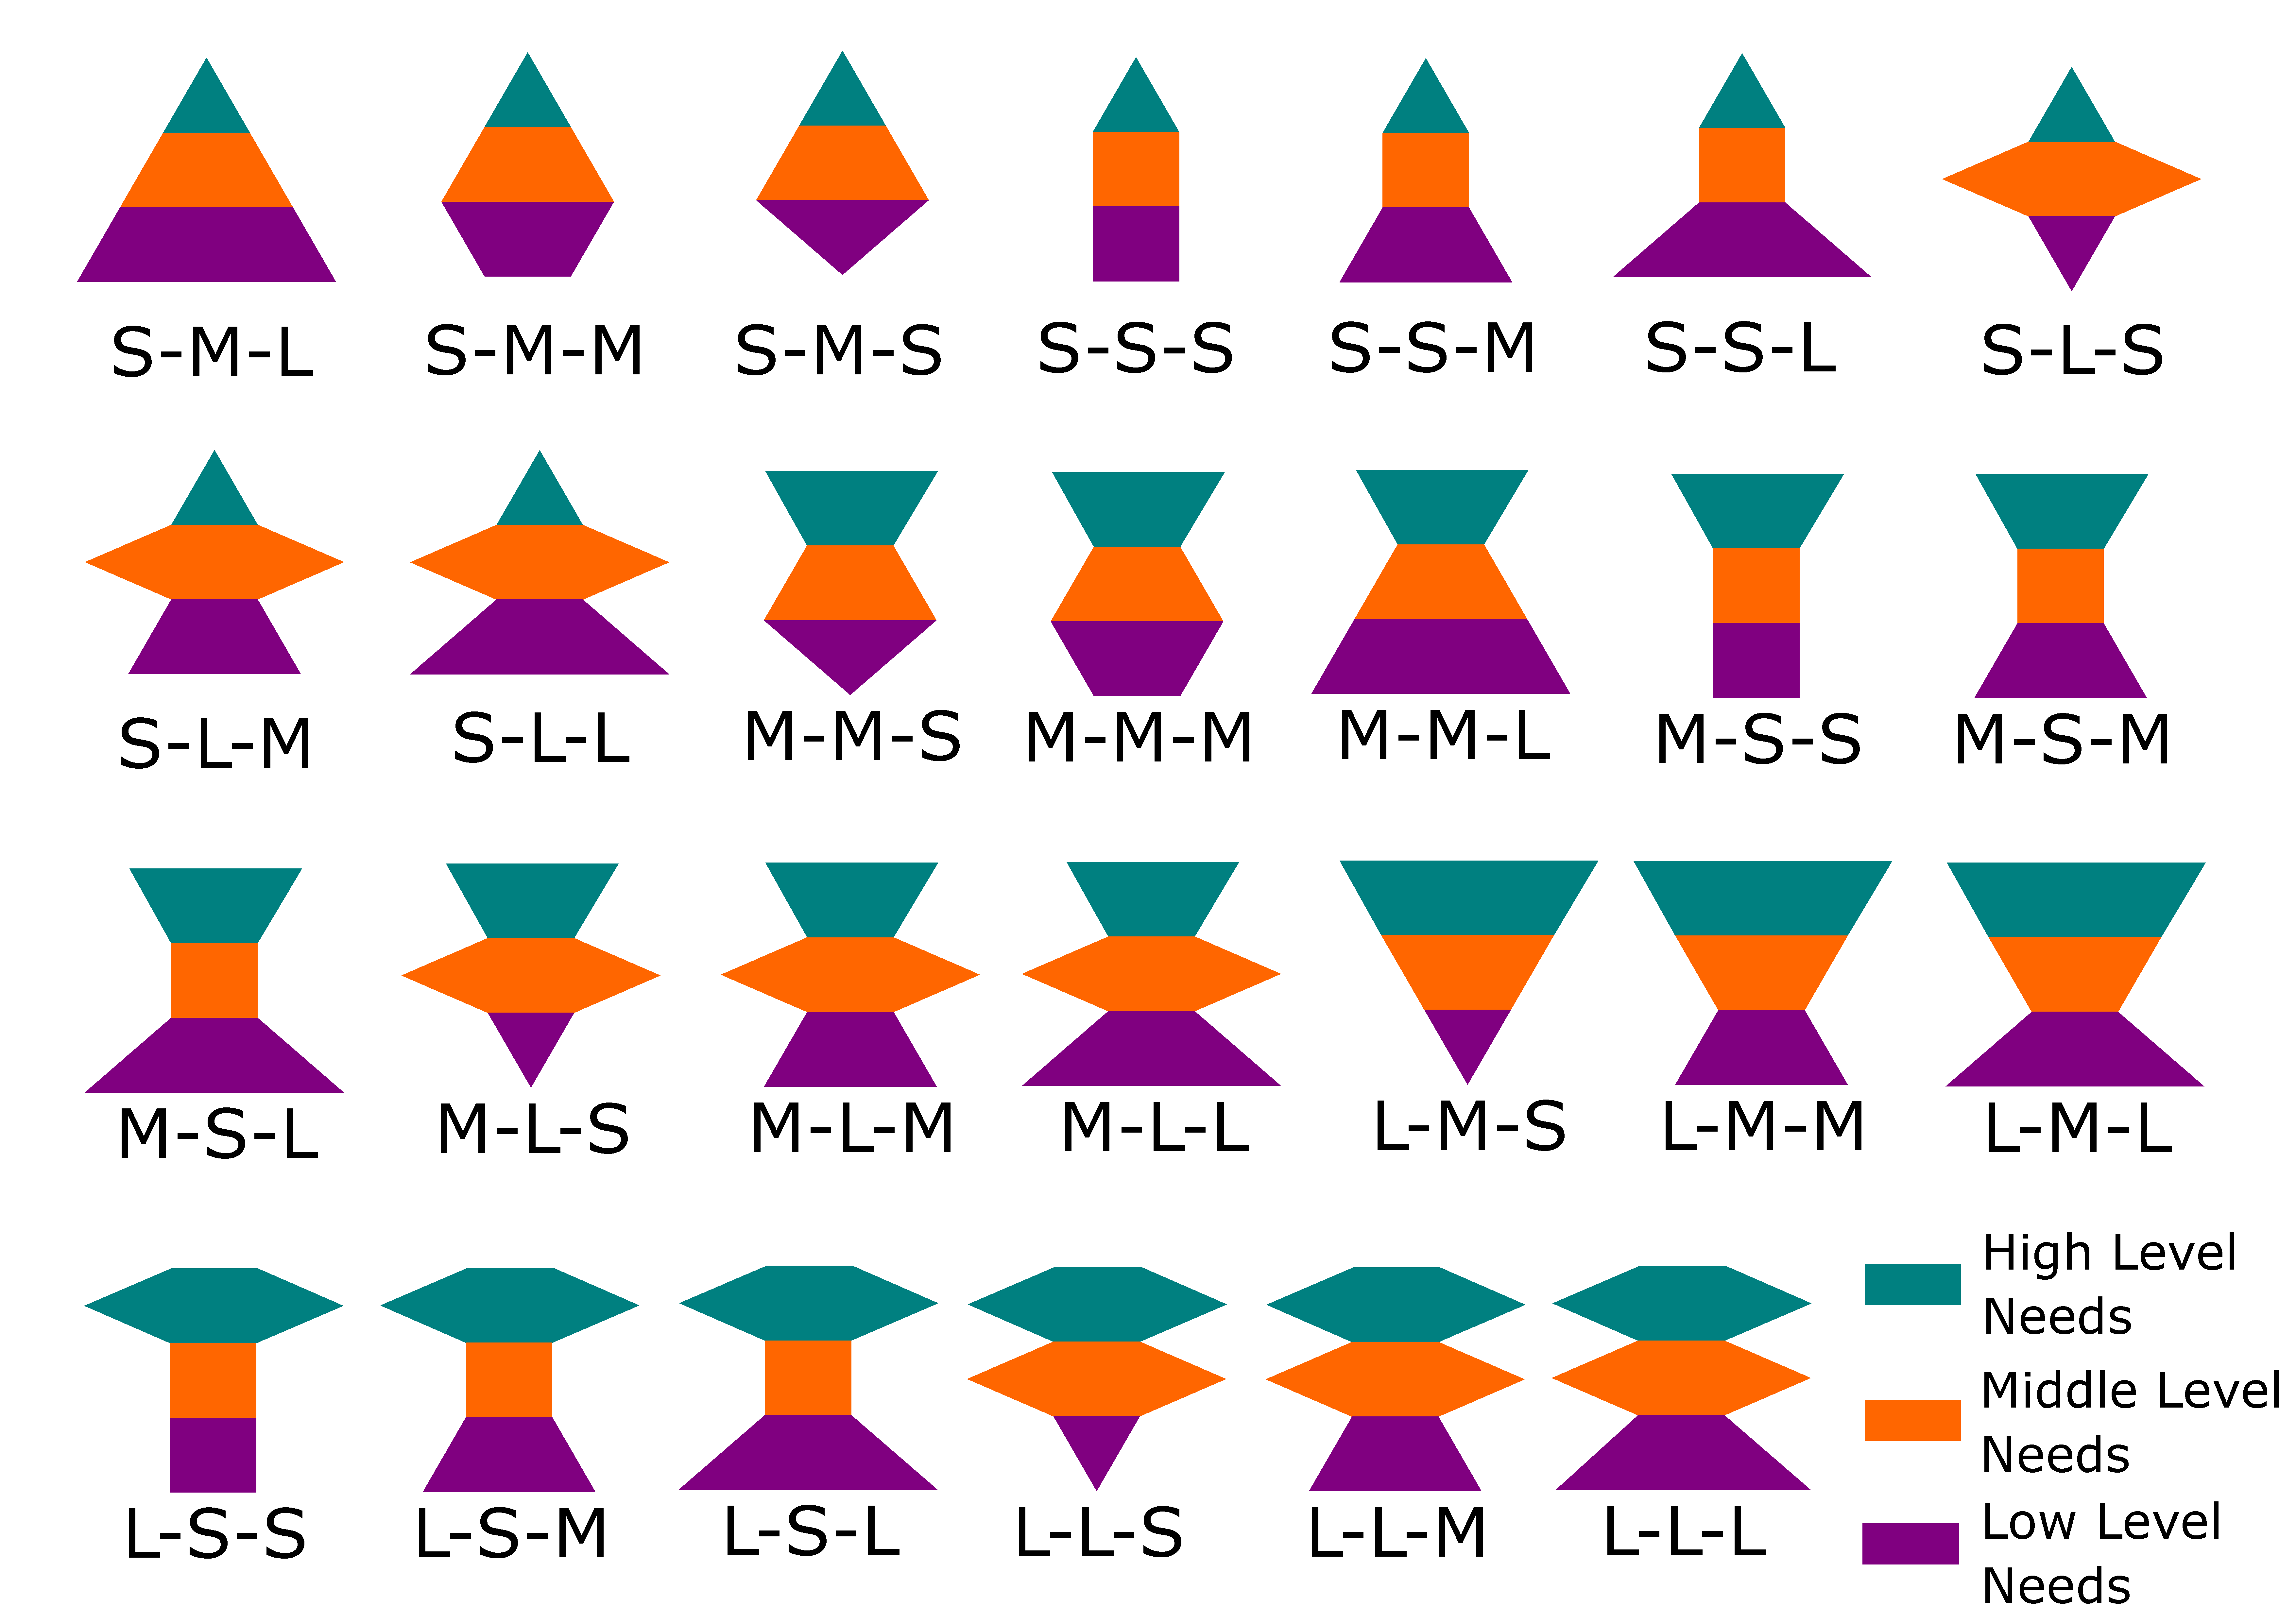
\includegraphics[width=1\columnwidth]{./figures/innate_values_models.pdf}
\caption{The illustration of innate values models with three-level needs of different amounts. \textit{S: Small; M: Medium; L: Large}}
\label{fig:overview}
\end{figure}

However, when we analyze natural agents, such as humans, they are usually combined motivation entities. They have biological motivations, including physiological, safety, and existence needs; social motivation, such as love and esteem needs; and cognitive motivation, like self-actualization or relatedness and growth needs \cite{merrick2009motivated}. The combined motivation theories include Maslow's Hierarchy of Needs \cite{maslow1958dynamic} and Alderfer's Existence Relatedness Growth (ERG) theory \cite{alderfer1972existence}. Fig. \ref{fig:overview} illustrates innate values (intrinsic motivations) models with three-level needs of different amounts.

Many researchers regard motivated behavior as behavior that involves the assessment of the consequences of behavior through learned expectations, which makes motivation theories tend to be intimately linked to theories of learning and decision-making \cite{baldassarre2013intrinsically}. In particular, intrinsic motivation leads organisms to engage in exploration, play, strategies, and skills driven by expected rewards. The computational theory of reinforcement learning (RL) addresses how predictive values can be learned and used to direct behavior, making RL naturally relevant to studying motivation.

In artificial intelligence, researchers propose various abstract computational structures to form the fundamental units of cognition and motivations, such as states, goals, actions, and strategies. For intrinsic motivation modeling, the approaches can be generally classified into three categories: prediction-based \cite{schmidhuber1991curious,schmidhuber2010formal}, novelty-based \cite{marsland2000real,merrick2009motivated}, and competence-based \cite{barto2004intrinsically,schembri2007evolution}. Furthermore, the concept of intrinsic motivation was introduced in machine learning and robotics to develop artificial systems learning diverse skills autonomously. The idea is that intelligent machines and robots could autonomously acquire skills and knowledge under the guidance of intrinsic motivations and later exploit such knowledge and skills to accomplish tasks more efficiently and faster than if they had to acquire them from scratch \cite{baldassarre2013intrinsically}. 

In other words, by investigating intrinsically motivated learning systems, we would clearly improve the utility and autonomy of intelligent artificial systems in dynamic, complex, and dangerous environments \cite{yang2023hierarchical,yang2022game}. Specifically, compared with the traditional RL model, intrinsically motivated RL refines it by dividing the environment into an external environment and an internal environment, which clearly generates all reward signals within the organism \footnote{Here, the organism represents all the components of the internal environment in the AI agent.} \cite{baldassarre2013intrinsically}. However, although the extrinsic reward signals are triggered by the objects and events of the external environment, and activities of the internal environment cause the intrinsic reward signals, it is hard to determine the complexity and variability of the intrinsic rewards (innate values) generating mechanism.

From the MAS perspective, learning in multi-agent settings is fundamentally more difficult than in the single-agent case due to the presence of multi-agent pathologies, e.g., the moving target problem (non-stationarity), curse of dimensionality, multi-agent credit assignment, global exploration, and relative overgeneralization \cite{hernandez2019survey}. Furthermore, due to each agent facing a moving-target learning issue, the best policy might change as the other agents modify their policies since all the agents are learning simultaneously in the process, which raises the nonstationarity of the multi-agent learning problem \cite{busoniu2008comprehensive}. Therefore, multi-agent RL algorithms need to balance exploiting the agent's current knowledge and exploring information-gathering actions to improve its knowledge. Especially for the cooperative MAS setting, individual choices of actions and strategies should be mutually consistent in order to achieve their common goals.

Moreover, most MAS implementations aim to optimize the system's policies with respect to individual needs and intrinsic values, even though many real-world problems are inherently multi-objective \cite{ruadulescu2020multi}. Thus, many conflicts and complex trade-offs in the MAS need to be managed, and compromises among agents should be based on the utility mapping the innate values of a compromise solution -- how to measure and what to optimize \cite{zintgraf2015quality}. However, in the MAS setting, the situations will become much more complex when we consider individual utility reflects its own needs and preferences \cite{yang2019self,yang2020hierarchical}. For example, although we assume each group member receives the same team rewards in fully cooperative MAS, the benefits received by an individual agent are usually significant differences according to its contributions and innate values in real-world scenarios or general multi-agent settings \cite{yang2023understanding}. 

To address those gaps, through integrating with combined motivation theories, we propose a novel innate-values-driven reinforcement learning (IVRL) model to describe the complex behaviors in MAS cooperation. By demonstrating the proposed architecture in the SAMC environment with three benchmark multi-agent RL algorithms (QMIX, IQL, and QTRAN), we prove that rationally organizing various individual needs can achieve better performance with lower costs in MAS cooperation effectively.

\section{Approach Overview}

\begin{figure}[t]
\centering
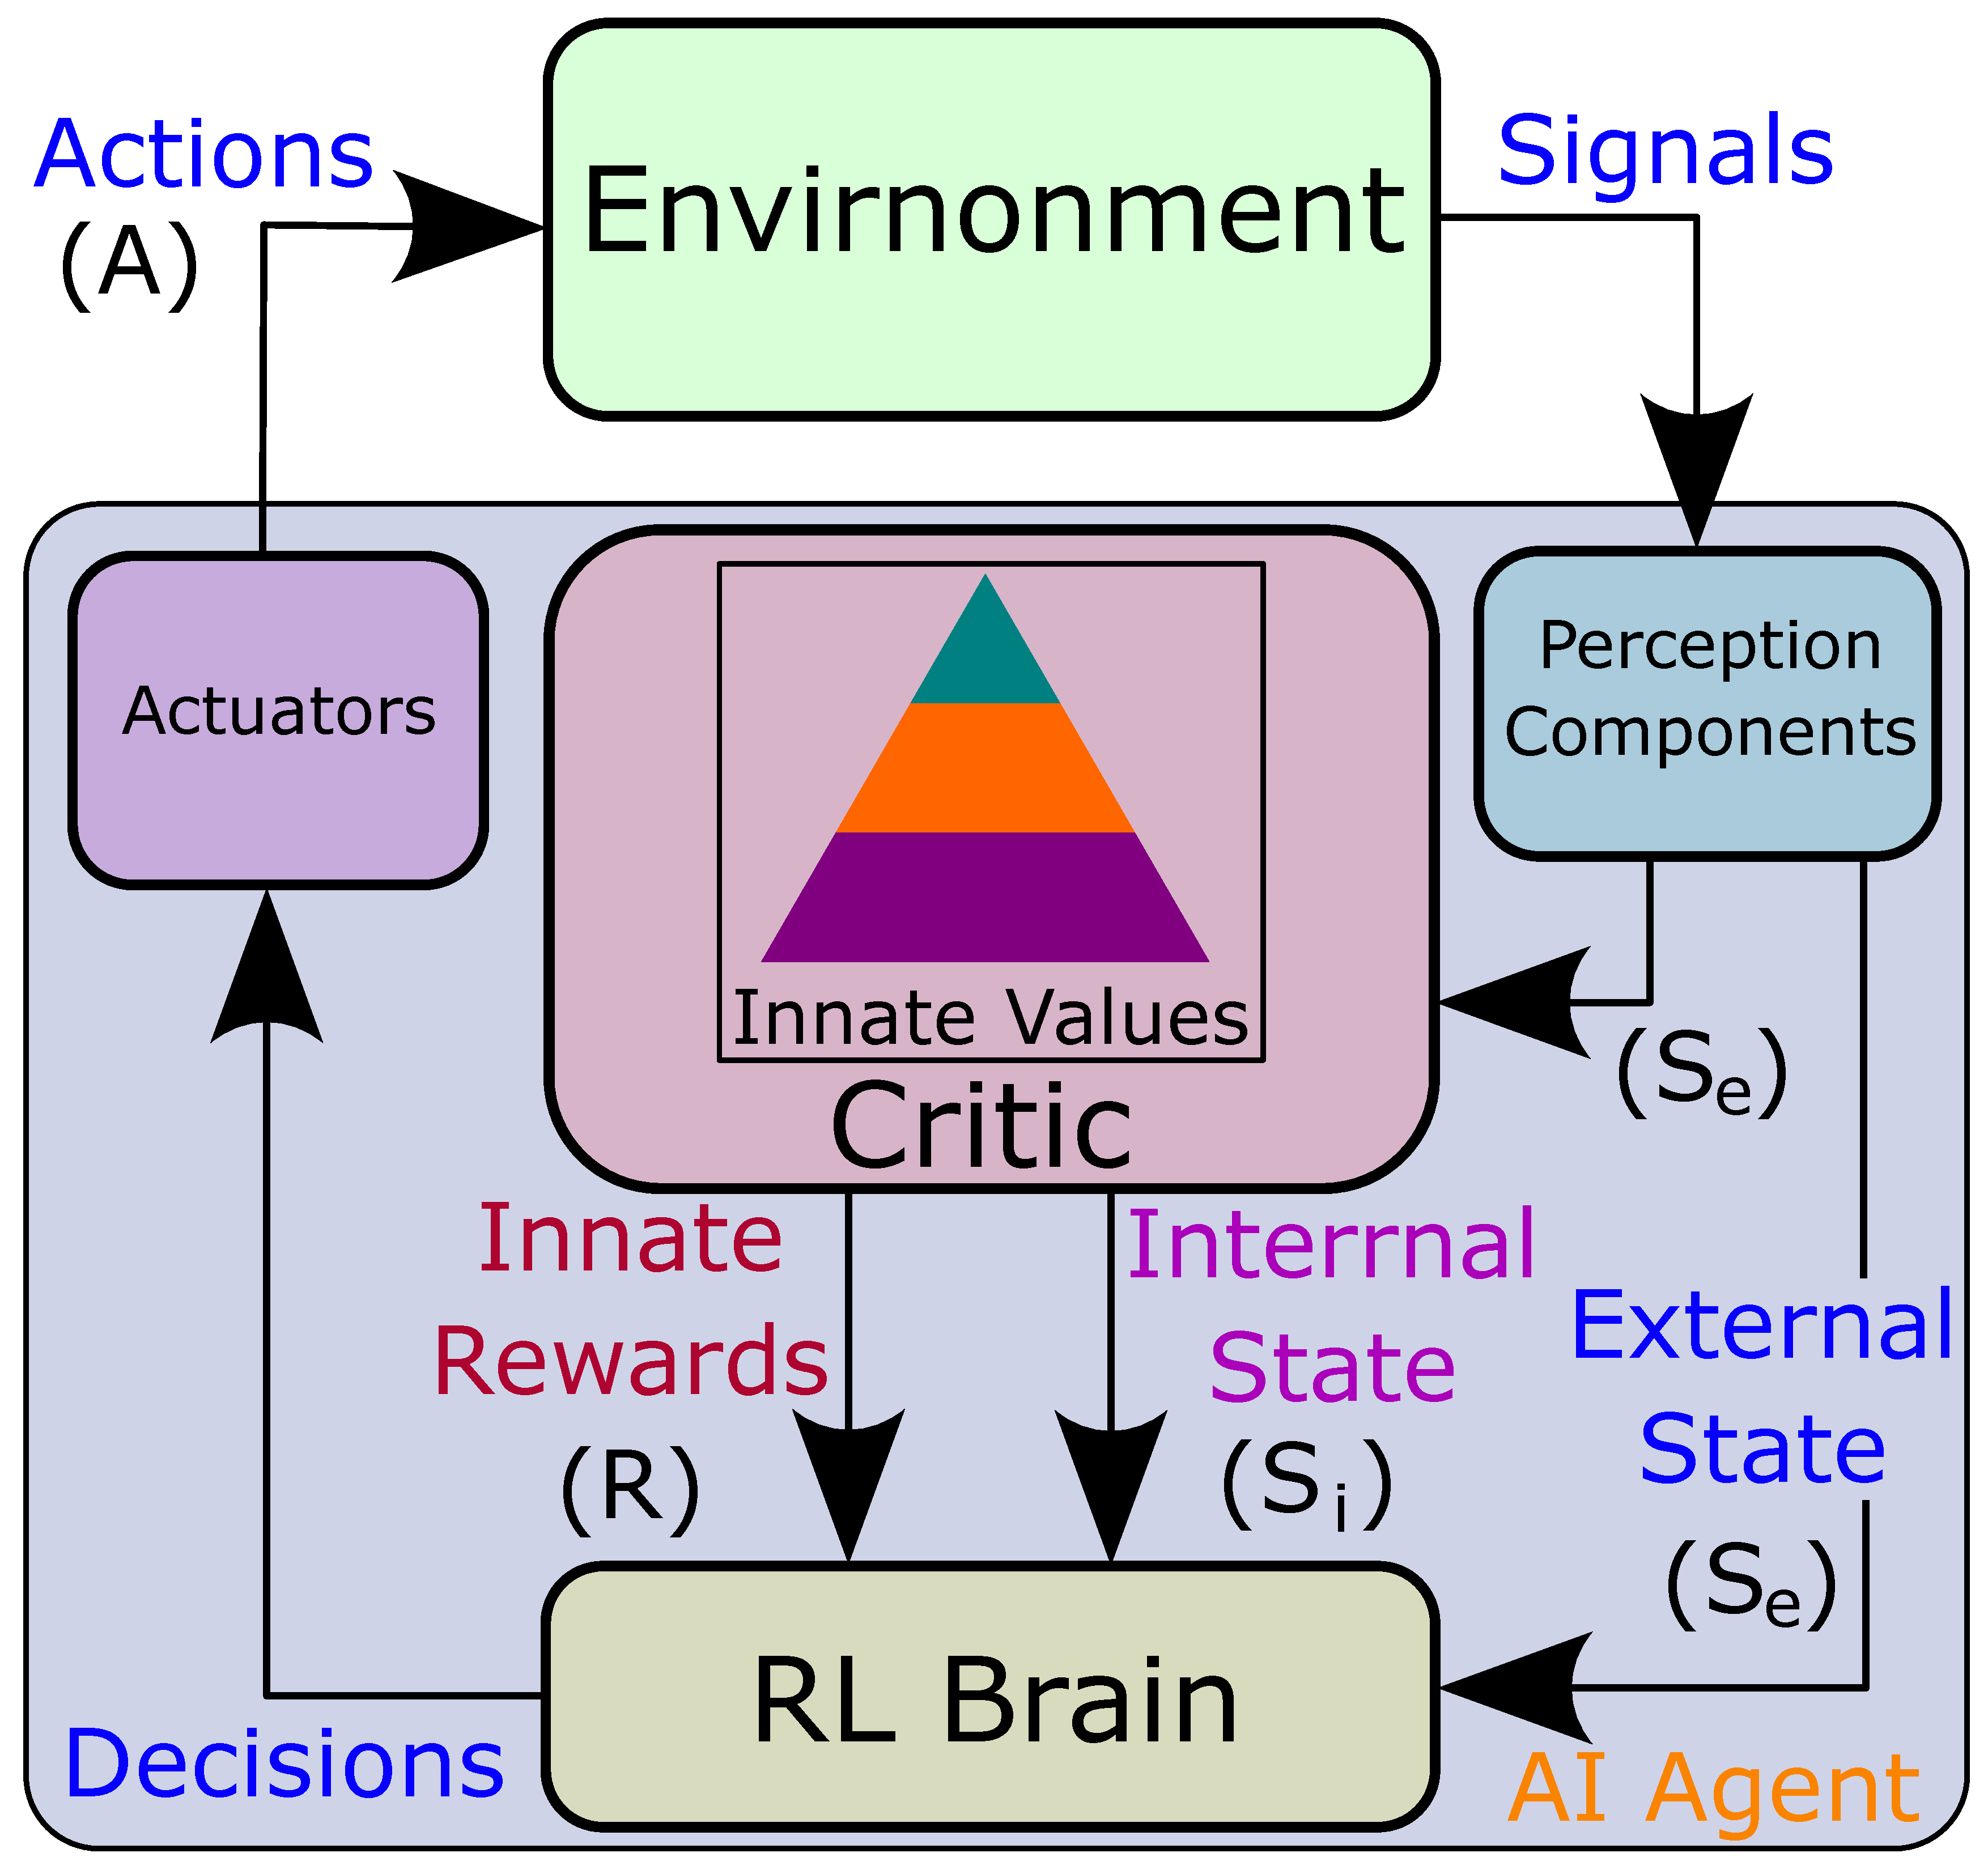
\includegraphics[width=0.85\columnwidth]{./figures/innate_values_RL_models.pdf}
\caption{The illustration of the proposed innate-values-driven reinforcement learning (IVRL) model.}
\label{fig:innate_values}
\end{figure}

We assume that all the AI agents (like robots) interact in the same working scenario, and their external environment includes all the other group members and mission setting. In contrast, the internal environment consists of individual perception components including various sensors (such as Lidar and camera), the critic module involving intrinsic motivation analysis and innate values generation, the RL brain making the decision based on the feedback of rewards and description of the current state (including internal and external) from the critic module, and actuators relating to all the manipulators and operators executing the RL brain's decisions as action sequence and strategies. Fig. \ref{fig:innate_values} illustrates the proposed IVRL model.

Compared with the traditional RL model, in our model, the input state and rewards are generated from the critic module instead of directly coming from the environment, which means that the individual needs to calculate benefits or utilities based on the innate value model and update its current internal status (the amount of the current needs locating in different levels) combining with external state sending to the RL model. For example, supposing two agents $a^1$ and $a^2$ have different innate value models: Fig. \ref{fig:overview} S-M-L and L-M-S. We use health points, energy levels, and task achievement to represent their safety needs $n_s$ (low-level intrinsic motivations), basic needs $n_b$ (middle-level intrinsic motivations), and teaming needs $n_t$ (High-level intrinsic motivations) \cite{yang2020needs,yang2021can,10.1145/3555776.3577642}, respectively. Considering $n_s^1 > n_s^2$, $n_b^1 = n_b^2$, and $n_t^1 < n_t^2$, if $a^1$ and $a^2$ receive the external repairing signal simultaneously, the innate rewards $r^1$ will larger than $r^2$ based on their innate value model (low-level safety needs $n_s^1 > n_s^2$). In contrast, if they get the order to collaborate with other agents fulfilling a task (high-level teaming needs $n_t^1 < n_t^2$) at the same time, the agent $a^2$ will receive more credits from it ($r^1 < r^2$). In other words, due to different innate value models, their intrinsic motivations present significant differences, which will lead to different innate rewards for performing the same task. Moreover, after calculating the practical credits for the individual utility in current actions, it will update its intrinsic status and combine with the external environment state sending to the RL model.

Furthermore, in the long term, the individual innate value model is dynamically changed after various needs at different levels are satisfied in the multi-agent interaction. It means that the agent's innate reward mechanism is not fixed, which helps it develop diverse skills and strategies to handle complex, multi-object, dynamic, and uncertain environments in the mission, similar to humans. Moreover, we formalize the proposed IVRL model as below.

\subsection{Single-Agent Systems}

In the single-agent systems, we formalize the IVRL of an AI agent with an external environment using a Markov decision process (MDP) \cite{puterman2014markov}. The MDP is defined by the tuple $\langle \mathcal{S, A, R, T,} \gamma \rangle$ where $\mathcal{S}$ represents the finite sets of internal state $S_i$\footnote{The internal state $S_i$ describes an agent's innate value distribution and presents the dominant intrinsic motivation based on the external state $S_e$.} and external states $S_e$. $\mathcal{A}$ represents a finite set of actions. The transition function $\mathcal{T}$: $\mathcal{S} \times \mathcal{A} \times \mathcal{S} \rightarrow$ [0, 1] determines the probability of a transition from any state $s \in \mathcal{S}$ to any state $s' \in \mathcal{S}$ given any possible action $a \in \mathcal{A}$. Assuming the critic function is $\mathcal{C}$, which describes the individual innate value model. The reward function $\mathcal{R} = \mathcal{C}(S_e): \mathcal{S} \times \mathcal{A} \times \mathcal{S} \rightarrow \mathbb{R}$ defines the immediate and possibly stochastic innate reward $\mathcal{C}(S_e)$ that an agent would receive given that the agent executes action $a$ which in state $s$ and it is transitioned to state $s', \gamma \in [0, 1)$ the discount factor that balances the trade-off between innate immediate and future rewards (Fig. \ref{fig:innate_values}).

The IVRL are adequate model to obtain optimal decisions in single agent fully observable environments. Solving the IVRL model will yield a policy $\pi: \mathcal{S} \rightarrow \mathcal{A}$, which is a mapping from internal and external state to actions. An optimal policy $\pi^*$ is the one that maximizes the expected discounted sum of innate rewards Eq. \eqref{expected_innate_rewards}. 
\begin{equation}
    \mathbb{E} \left[\sum_{t \geq 0} \gamma^t \mathcal{C}(s_{i_t}, a_t, s_{i_{t+1}}) \bigg\vert a_t \sim \pi(\cdot \vert s_t), s_0 \right]
\label{expected_innate_rewards}
\end{equation}

Accordingly, we can define the \textit{action-innate-value} function (Q-function) and \textit{state-innate-value} function (V-function) under policy $\pi$ as Eq. \eqref{q_innate_rewards} and \eqref{v_innate_rewards} for any $s \in \mathcal{S}$ and $a \in \mathcal{A}$, which are the discounted accumulated innate reward starting from $(s_0, a_0) = (s, a)$ and $s_0 = s$, respectively.
\begin{equation}
\begin{split}
    & \mathbf{Q}_\pi (s, a) = \\
    & \mathbb{E} \left[\sum_{t \geq 0} \gamma^t \mathcal{C}(s_{i_t}, a_t, s_{i_{t+1}}) \bigg\vert a_t \sim \pi(\cdot \vert s_t), a_0 = a, s_0 = s \right]
\label{q_innate_rewards}
\end{split}
\end{equation}
\begin{equation}
\begin{split}
    \mathbf{V}_\pi (s, a) & = \\
    & \mathbb{E} \left[\sum_{t \geq 0} \gamma^t \mathcal{C}(s_{i_t}, a_t, s_{i_{t+1}}) \bigg\vert a_t \sim \pi(\cdot \vert s_t), s_0 = s \right]
\label{v_innate_rewards}
\end{split}
\end{equation}

Here, the ones corresponding to the optimal policy $\pi^*$ are referred to as the optimal Q-function and the optimal state-innate-value function, respectively.

\subsection{Multi-Agent Systems}

In the multi-agent setting, we consider the Markov games, also known as stochastic games \cite{shapley1953stochastic}, originating from the seminal work \cite{littman1994markov}. We formalize the IVRL of the MAS as below:

A Markov game is defined by a tuple $(\mathcal{N}$, $\mathcal{S}$, $\{\mathcal{A}^i\}_{i \in \mathcal{N}}$, $\mathcal{P}$, $\{\mathcal{R}^i\}_{i \in \mathcal{N}}$, $\gamma)$, where $\mathcal{N}$ = $\{1, \dots, N \}$ denotes the set of $N > 1$ agents, $\mathcal{A}^i$ denotes the action space of agent $i$. Let $\mathcal{A} := \mathcal{A}^1 \times \cdots \times \mathcal{A}^N$, then $\mathcal{P}: \mathcal{S} \times \mathcal{A} \rightarrow \Delta(\mathcal{S})$ denotes the transition probability from any state $s \in \mathcal{S}$ to any state $s' \in \mathcal{S}$ (including internal state $\mathcal{S}_i$ and external state $\mathcal{S}_e$) for any joint action $a \in \mathcal{A}$. For the agent $i$, $\mathcal{C}^i$ is the critic function of the innate value model. $\mathcal{R}^i = \mathcal{C}^i(\mathcal{S}_e^i): \mathcal{S} \times \mathcal{A} \times \mathcal{S} \rightarrow \mathbb{R}$ is the innate reward function that determines the immediate reward received by agent $i$ for a transition from $(s, a)$ to $s'$. $\gamma \in [0, 1)$ is the discount factor.

Any time $t$, each agent $i \in \mathcal{N}$ executes an action $a_t^i$, according to the system state $s_t$. The system then transitions to state $s_{t+1}$, and innate rewards of each agent $i$ by $\mathcal{R}^i = \mathcal{C}^i(s_{i_t}, a_t, s_{i_{t+1}})$. The goal of agent $i$ is to optimize its own long-term innate reward, by finding policy $\pi^i: \mathcal{S} \rightarrow \Delta(\mathcal{A}^i)$ such that $a_t^i \dim \pi^i(\cdot \vert s_t)$. As a consequence, the innate value function $V^i: \mathcal{S}_i \rightarrow \mathbb{R}$ of agent $i$ becomes a function of joint policy $\pi: \mathcal{S} \rightarrow \Delta(\mathcal{A})$ defined as $\pi(a \vert s):= \prod_{i \in \mathcal{N}} \pi^i(a^i \vert s)$. In particular, for any joint policy $\pi$ and state $s \in \mathcal{S}$, we can get Eq. \eqref{mv_innate_rewards}, where $-i$ represents the indices of all agents in $\mathcal{N}$ except agent $i$.
\begin{equation}
\begin{split}
    & \mathbf{V}_{\pi^i, \pi^{-i}}^i (s) := \\
    & \mathbb{E} \left[\sum_{t \geq 0} \gamma^t \mathcal{C}^i(s_{i_t}, a_t, s_{i_{t+1}}) \bigg\vert a_t^i \sim \pi^i(\cdot \vert s_t), s_0 = s \right]
\label{mv_innate_rewards}
\end{split}
\end{equation}

Here, the optimal performance of each agent is controlled not only by its own policy but also by the choice of all other group members of the game.

\subsection{Cooperative Setting}

In the IVRL model, the innate value function describes the agent's current motivation status and dominant motivation. If agents have similar distributions of needs or motivations, they will share a common innate value function, i.e., $\mathcal{C}^1 = \mathcal{C}^2 = \cdots = \mathcal{C}^\mathcal{N}$, which means that they have the potential to collaborate in the current situation \cite{yang2021can}. Moreover, from the game-theoretic perspective, if all agents' innate value functions and Q-functions are identical, they can be coordinated as one decision-maker, and the global optimum for cooperation now constitutes a Nash equilibrium of the game.

However, the innate value distributions of agents will dynamically change (Fig. \ref{fig:overview}) due to satisfying individuals' current needs and motivations. In the long term, in order to optimize the global system’s utility and guarantee sustainable development for each group member, we can dynamically group the agents of similar innate value models and assign them corresponding tasks. Moreover, we can optimize the average innate reward $\bar{\mathcal{C}}(s_e, a, s'_e) := \mathcal{N}^{-1} \cdot \sum_{i \in \mathcal{N}} \mathcal{C}^i(s_e, a, s'_e)$, which allow to have different innate reward functions and more heterogeneity among agents (agents with different motivations and needs), similar to human society.

\section{Evaluation through Simulation Studies}

\begin{figure*}[hptb]
\centering

\includegraphics[width=\textwidth]{./figures/smac.png}
\caption{Illustration of the 2s3z Map in the StarCraft II Multi-Agent Challenge (SMAC) Experiment Environment}
\label{fig:smac}
\end{figure*}
\begin{figure*}[hptb]
\subfigure[Battle Won Mean (QMIX)]{
\label{fig:qmix_bw}
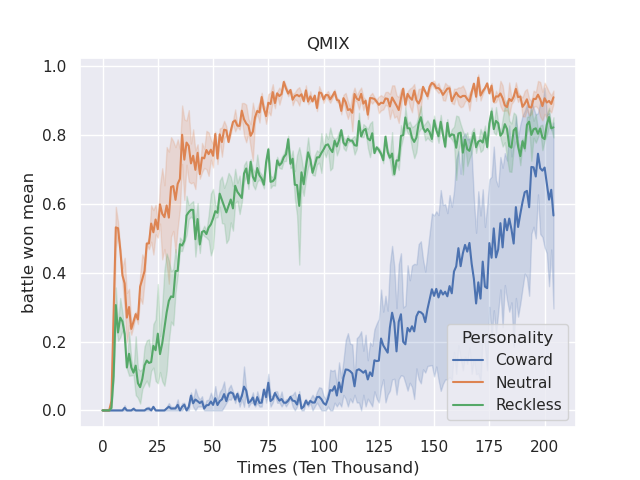
\includegraphics[width=0.325\textwidth]{./figures/qmix_battle_won_mean.png}}
\subfigure[Dead Allies Mean (QMIX)]{
\label{fig:qmix_da}
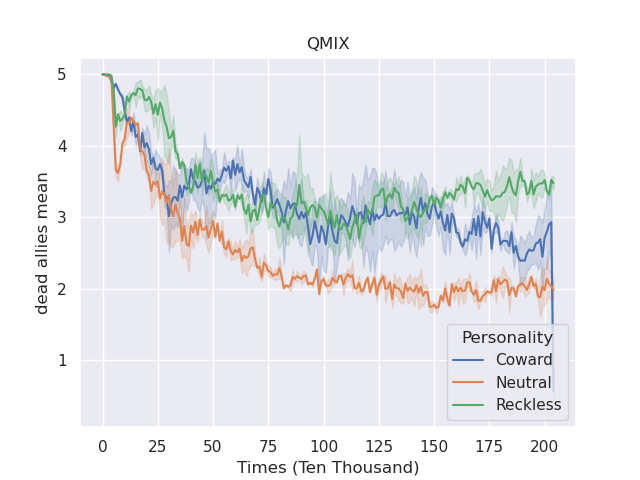
\includegraphics[width=0.325\textwidth]{./figures/qmix_dead_allies_mean.png}}
\subfigure[Dead Enemies Mean (QMIX)]{
\label{fig:qmix_de}
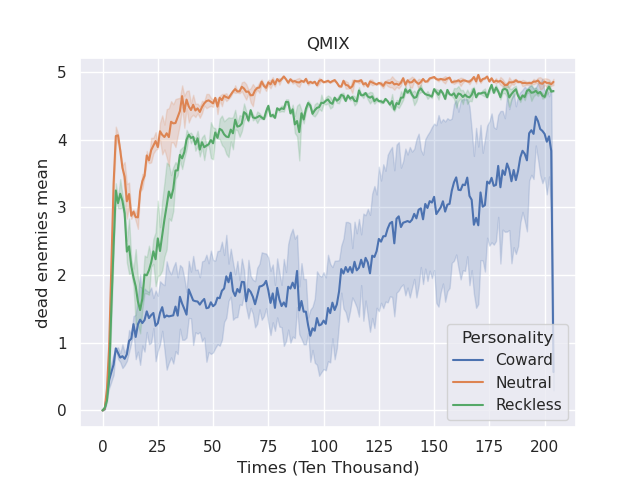
\includegraphics[width=0.325\textwidth]{./figures/qmix_dead_enemies_mean.png}}
% \vspace{-4mm}
% \caption{The group performance of three personalities (innate-value) agents with QMIX in the SMAC (Map: 2s3z)}
% \label{bsn_gym}
% \end{figure*}
% \begin{figure*}[tbp]
\centering
\subfigure[Battle Won Mean (IQL)]{
\label{fig:iql_bw}
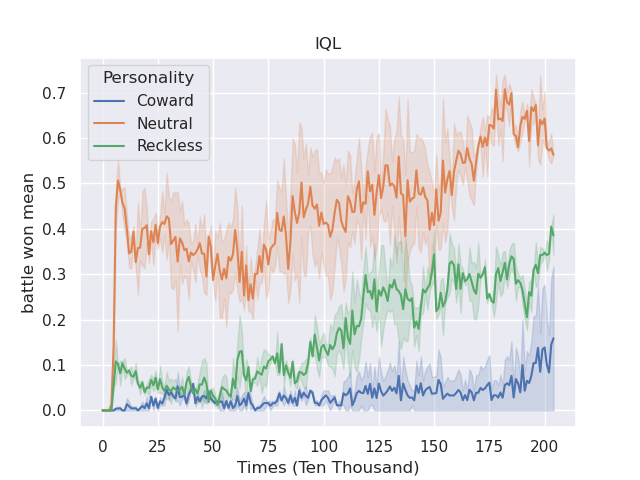
\includegraphics[width=0.325\textwidth]{./figures/iql_battle_won_mean.png}}
\subfigure[Dead Allies Mean (IQL)]{
\label{fig:iql_da}
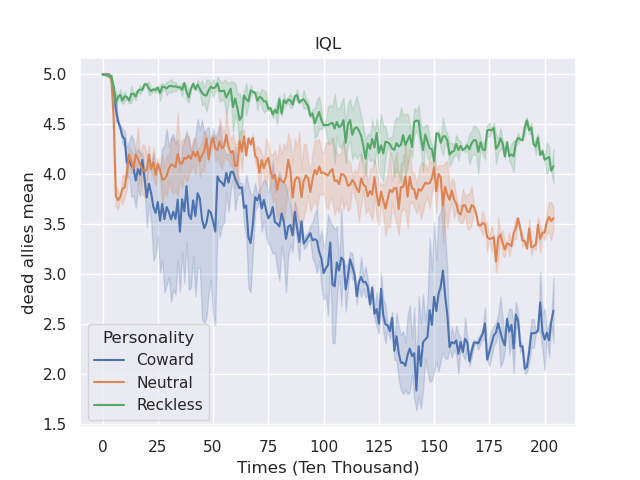
\includegraphics[width=0.325\textwidth]{./figures/iql_dead_allies_mean.png}}
\subfigure[Dead Enemies Mean (IQL)]{
\label{fig:iql_de}
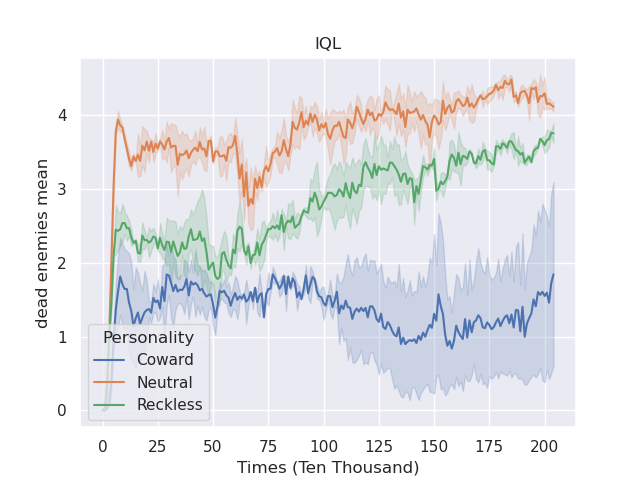
\includegraphics[width=0.325\textwidth]{./figures/iql_dead_enemies_mean.png}}
% \vspace{-4mm}
% \caption{The group performance of three personalities (innate-value) agents with IQL in the SMAC (Map: 2s3z)}
% \label{bsn_gym}
% \end{figure*}
% \begin{figure*}[tbp]
\centering
\subfigure[Battle Won Mean (QTRAN)]{
\label{fig:qtran_bw}
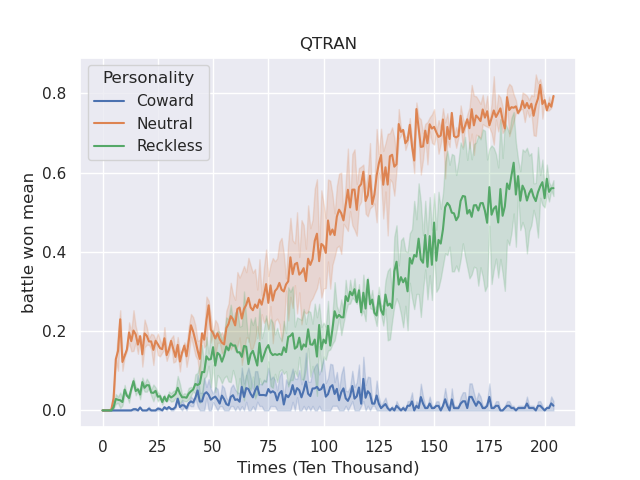
\includegraphics[width=0.325\textwidth]{./figures/qtran_battle_won_mean.png}}
\subfigure[Dead Allies Mean (QTRAN)]{
\label{fig:qtran_da}
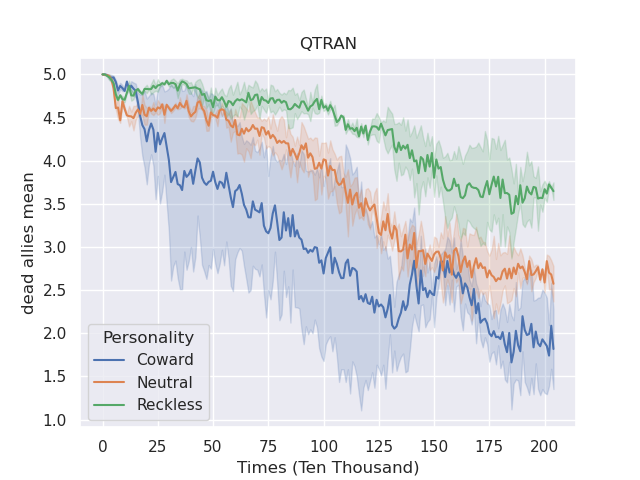
\includegraphics[width=0.325\textwidth]{./figures/qtran_dead_allies_mean.png}}
\subfigure[Dead Enemies Mean (QTRAN)]{
\label{fig:qtran_de}
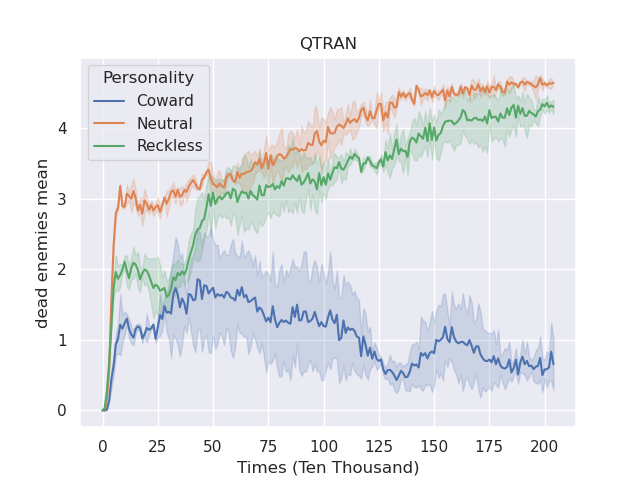
\includegraphics[width=0.325\textwidth]{./figures/qtran_dead_enemies_mean.png}}
% \vspace{-4mm}
\caption{The group performance of three personalities (innate-value) agents with QMIX, IQL, and QTRAN in the SMAC}
\label{results}
\end{figure*}

We evaluate the performance of the proposed innate-value-driven reinforcement learning (IVRL) model in the StarCraft Multi-Agent Challenge (SMAC) \cite{samvelyan19smac} environment. Our experiments define three types of group agents based on the proposed innate-value model\footnote{This experiment only consider static innate-value system setting.}, which presents corresponding group personalities: \textit{Coward}, \textit{Neutral}, and \textit{Reckless}. 
Furthermore, we study the group performance of different characteristics in several benchmark multi-agent RL algorithms, such as QMIX \cite{rashid2020monotonic}, IQL \cite{tampuu2017multiagent}, and QTRAN \cite{son2019qtran}. And we discuss more details as below.

\subsection{Experiment Setting}

In our experiment, we use a weight matrix to model the reward mechanism of the innate value system. To simplify the computational process, we only consider three factors -- battle won (BW), shield level (SL), and health points (HP) -- (Eq. \eqref{weight_matrix}) describing the innate value distribution of an agent.
\begin{equation}
\begin{split}
    \mathbb{W}_{iv} = \left [ 
    \begin{aligned}
    & \mathbf{Achievement}_{high\_level\_needs} \\
    & \mathbf{Safety}_{middle\_level\_needs} \\
    & \mathbf{Basic}_{low\_level\_needs}
    \end{aligned}
    \right ] = 
    \left [ 
    \begin{aligned}
    & \mathcal{BW}_{weight} \\
    & \mathcal{SL}_{weight}  \\
    & \mathcal{HP}_{weight}
    \end{aligned}
    \right ]
\label{weight_matrix}
\end{split}
\end{equation}

Specifically, according to the Eq. \eqref{weight_matrix}, we define the agent of the coward, neutral, and reckless based on different innate value weights in the matrix, which express distinguished rewards with the same actions or strategies when it interacts with the environments and other agents. For example, the coward cares much about its life and HP. On the other hand, the reckless only eyes on the result of the battle won regardless of its life and safety. Compared with the two types of agents, the neutral agent represents more rationality to balance the low-level basic and safety needs and high-level teaming needs (battle won). Moreover, we can formalize the coward (Eq. \eqref{coward}), neutral (Eq. \eqref{neutral}), and reckless (Eq. \eqref{reckless}) as follow:
\begin{eqnarray}
    & \mathcal{BW}_{weight} \ll \mathcal{SL}_{weight} \approx \mathcal{HP}_{weight}; \label{coward} \\
    & \mathcal{BW}_{weight} \approx \mathcal{SL}_{weight} \approx \mathcal{HP}_{weight}; \label{neutral} \\
    & \mathcal{BW}_{weight} \gg \mathcal{SL}_{weight} \approx \mathcal{HP}_{weight}; \label{reckless}
\end{eqnarray}

Considering integrating the agent's parameters of the StatCraft II into the individual innate-value system, we also use the corresponding health points and shield level representing its basic and safety needs, respectively. Moreover, we apply the result of the battle won for each episode to describe the teaming goal as the individual high-level needs achieving in their cooperation. We implement three benchmark multi-agent RL algorithms, such as QMIX, IQL, and QTRAN, in the standard StarCraft map 2s3z to evaluate the battle performance of the three types group of agents (Eq. \eqref{coward}, \eqref{neutral}, and \eqref{reckless}). Furthermore, we list the innate-value weight matrix of each type of agent in corresponding experiments as Tab. \ref{tab:weight_matrix}. Fig. \ref{fig:smac} illustrates the 2s3z testing Map in the StarCraft II Multi-Agent Challenge (SMAC) Experiment Environment.

\begin{table}[h]
% \vspace{-2mm}
 \renewcommand\arraystretch{1.5}
 \caption{\small{Innate-Value Weight Matrix of Each Type of Agent in Experiments.}}
    \label{tab:weight_matrix}
\resizebox{\columnwidth}{!}{\begin{tabular}{|c|c|c|c|}
%\scriptsize
    \hline
    \diagbox{ALG}{Weight Matrix}{CHAR} & Coward & Neutral & Reckless \\ \hline
    QMIX & [1, -2.5, -2.5]$^T$ & [1, -1, -1]$^T$ & [1, 2.5, 2.5]$^T$ \\ 
    \hline
    IQL & [1, -2.5, -2.5]$^T$ & [1, -1, -1]$^T$ & [1, 2.5, 2.5]$^T$ \\ 
 \hline
    QTRAN & [1, -3, -3]$^T$ & [1, -1, -1]$^T$ & [1, 3, 3]$^T$ \\ 
 \hline
 \end{tabular}}
% \vspace{-3mm}
\end{table}

Generally, different characteristic agents present unique innate-value systems corresponding to the specific reward mechanism to interact with other agents and various environments.

\subsection{Evaluation and Results}

We first study the proposed IVRL architecture with the QMIX algorithm. Fig. \ref{fig:qmix_bw} shows that the group of neutral agents has the highest battle-won mean compared with the reckless group and coward group. For the innate-value system of cowards, since they care more about low-level needs, like basic and safety needs, their personality presents a kind of self-interest in the battle. It means selfishness and greedy behaviors can achieve more rewards in their value systems. Therefore, these individual behaviors significantly damage the benefits of the entire group and hinder the team's cooperation to fulfill the task and reach high-level goals. Moreover, since group benefits have been seriously damaged, it has impacted individual interests substantially. Fig. \ref{fig:qmix_da} and \ref{fig:qmix_de} demonstrate that the coward group loses more allies but destroys fewer enemies.
 
In contrast, although the reckless group focuses on the high-level group achievement of winning the battle, it costs many agents due to ignoring the individual low-level basic and safety needs (Fig. \ref{fig:qmix_da} and \ref{fig:qmix_de}). It also affects the group to achieve better performance (Fig. \ref{fig:qmix_bw}). Furthermore, the neutral group represents more rational behaviors in the battle, balancing the team's and individual interests. In other words, based on the reward mechanism of the innate value system, the neutral agents optimize the global system’s utility and guarantee sustainable development for each group member by balancing the rewards between agents and groups in MAS cooperation, much like human society does.

Furthermore, we implement the algorithms of IQL and QTRAN in the IVRL architecture. They all show similar results as the QMIX (Fig. \ref{fig:iql_bw} and \ref{fig:qtran_bw}). Especially in the Fig. \ref{fig:iql_da} and \ref{fig:qtran_da}, they illustrate that the coward group's behaviors can save more allies' lives, but the reckless group's behaviors cost a lot.

Generally, the innate value system serves as a unique reward mechanism driving agents to develop diverse actions or strategies satisfying their various needs in the systems. It also builds different personalities and characteristics of agents in their interaction. Moreover, organizing agents with similar interests and innate values in the mission can optimize the group utilities and reduce costs effectively, just like ``Birds of a feather flock together." in human society.

\section{Conclusion and Future Works}

This paper introduces the innate-values-driven reinforcement learning (IVRL) model mimicking the complex behaviors of different characteristic multi-agent interactions in cooperation. For theoretical derivation, we formulate the IVRL model within different scenarios, such as single-agent, multi-agent, and cooperative settings. Furthermore, we demonstrate the proposed architecture in the SAMC environment with three benchmark multi-agent RL algorithms (QMIX, IQL, and QTRAN). The results prove that rationally organizing various individual needs can achieve better performance with lower costs in MAS cooperation effectively.

For future work, we want to improve the IVRL further and develop a more comprehensive system to personalize individual characteristics to achieve various tasks testing in several standard MAS testbeds, such as StarCraft II, OpenAI Gym, Unity, etc. Moreover, integrating efficient deep RL algorithms, such as BSAC \cite{yang2023strategy,yang2022bsac}, with the IVRL can help agents evolve diverse skills to adapt to complex environments in MAS cooperation. Furthermore, implementing the IVRL in real-world systems, such as human-robot interaction, multi-robot systems, and self-driving cars, would be challenging and exciting.

% \clearpage

\bibliography{aaai24}

\end{document}
